\documentclass[12pt]{article}

\usepackage{eamc-template}

\usepackage[round,sort]{natbib}
\usepackage[brazil]{babel}   
\usepackage[latin1]{inputenc}
\usepackage{graphicx,url}
\usepackage{float}
\usepackage{tabularx}
\usepackage{booktabs}
\usepackage{blindtext}
     
\sloppy

\title{Template EAMC: Um exemplo can�nico}

\author{Diego T. Volpatto\inst{1}, Marianna N. Martins\inst{2}, Camila M. Saporetti\inst{3}}


\address{Laborat�rio Nacional de Computa��o Cient�fica (LNCC)\\
  Caixa Postal 25.651-075 -- Petr�polis, RJ -- Brasil
\nextinstitute
  Instituto de Computa��o -- Universidade Estadual de Campinas (IC-UNICAMP)\\
  Campinas, SP -- Brasil
\nextinstitute
  Universidade Federal de Juiz de Fora (UFJF) \\ 
  Juiz de Fora, MG -- Brasil
  \email{volpatto@lncc.br, m163115@g.unicamp.br,
  camilasaporetti@ice.ufjf.br}
}

\begin{document} 

\maketitle

\begin{abstract}
\blindtext
\end{abstract}
     
\begin{resumo} 
\blindtext
\end{resumo}

\section{Uma Se��o}

\blindtext

\section{Outra Se��o} \label{sec:firstpage}

\blindtext

\subsection{Uma Subse��o}

\blindtext

\subsubsection{Uma Subsubse��o}

\blindtext

\section{Figuras e Tabelas}\label{sec:figs}

Segue exemplos de figuras:

\begin{figure}[!ht]
\centering
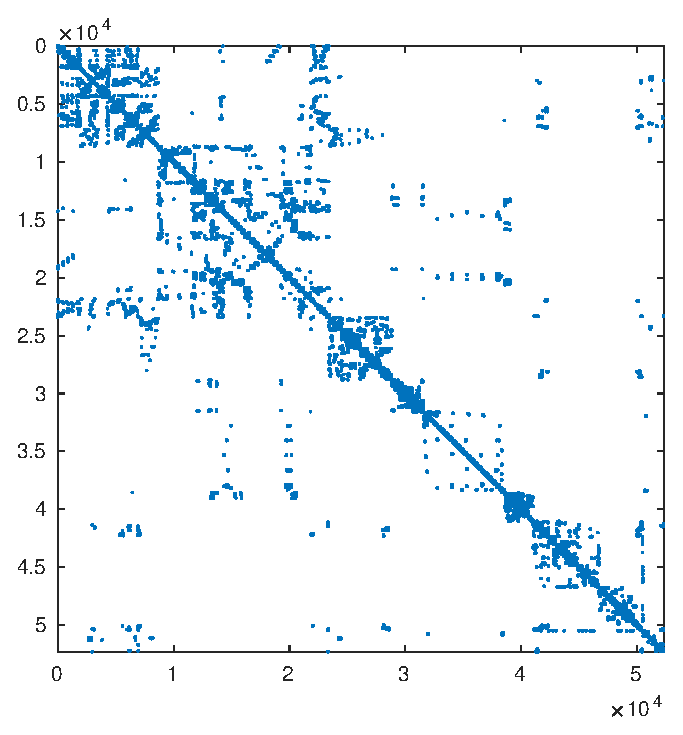
\includegraphics[width=.5\textwidth]{./figuras/A}
\caption{Uma figura.}
\label{fig:exampleFig1}
\end{figure}

\begin{figure}[H]
\centering
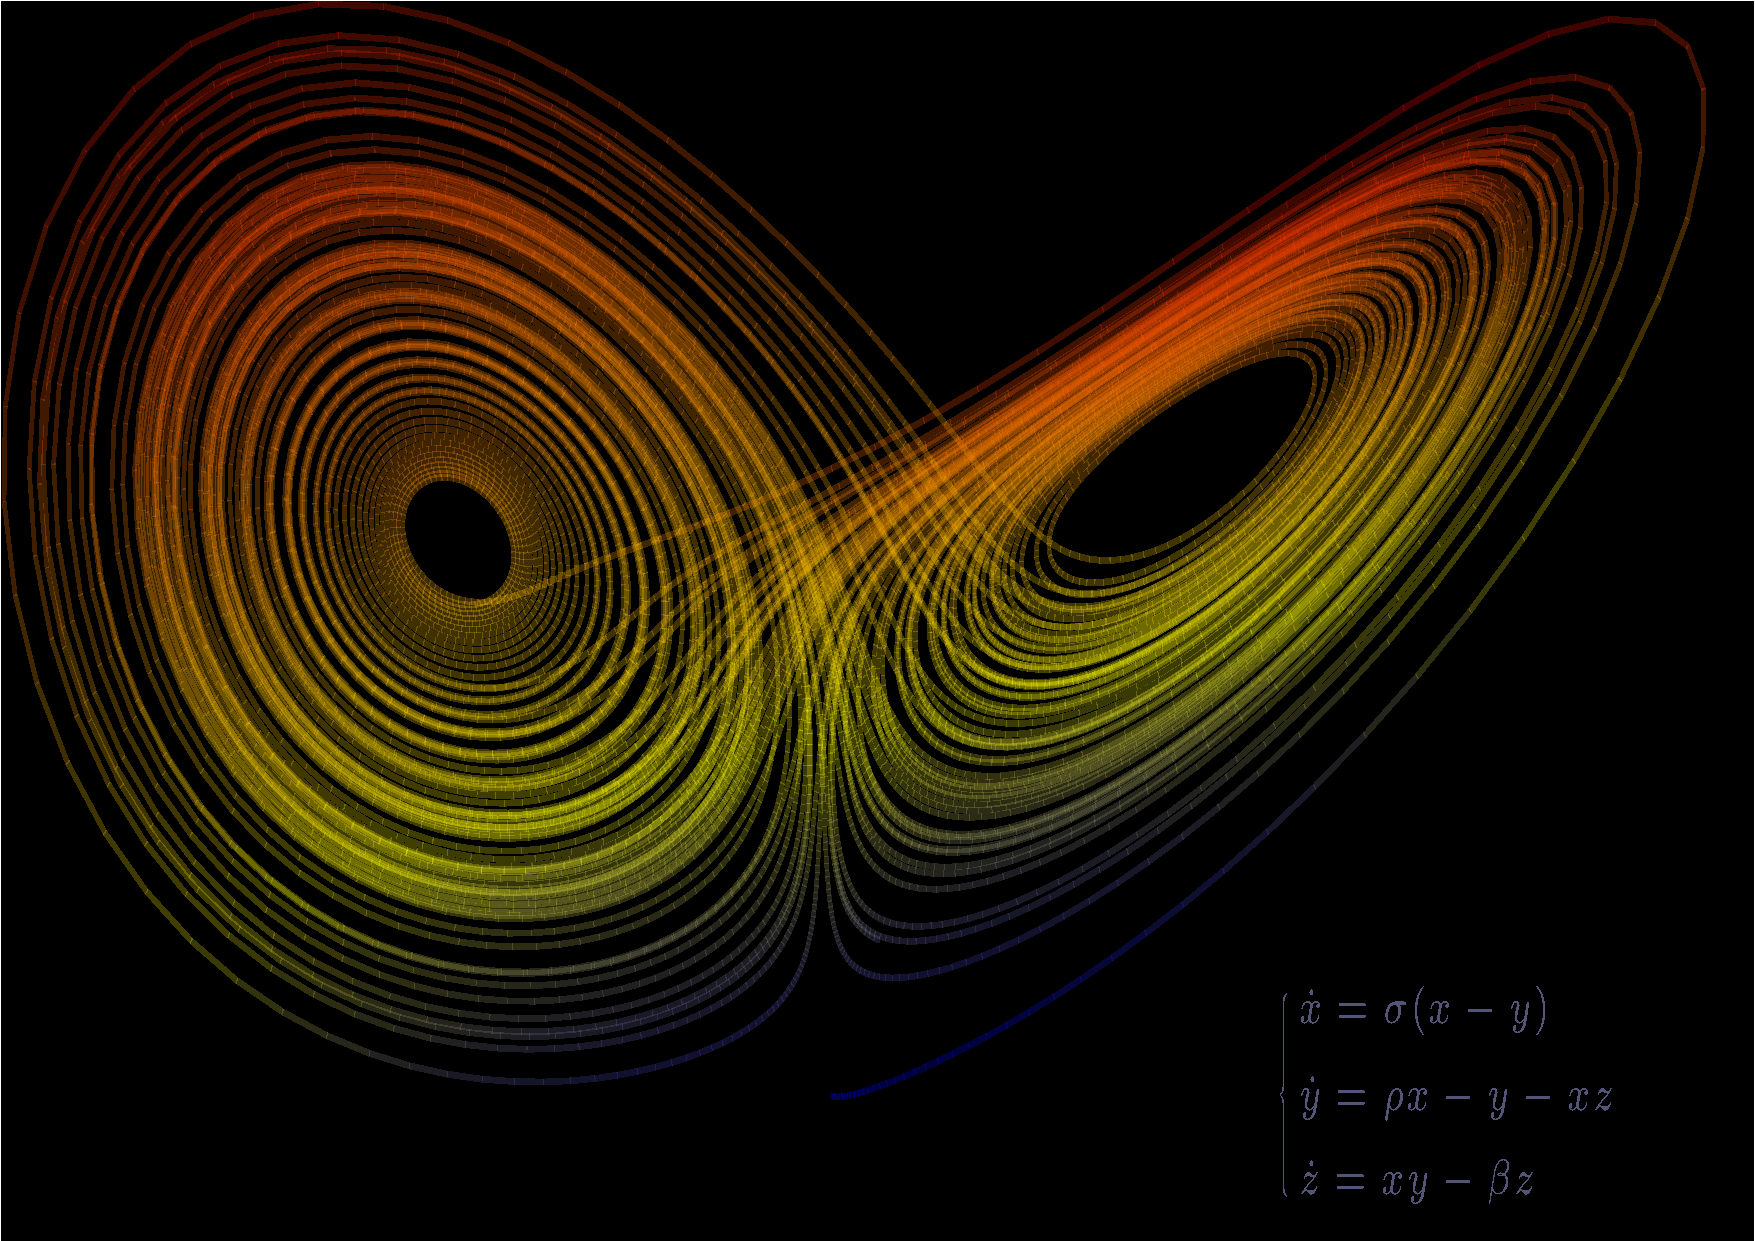
\includegraphics[width=.5\textwidth]{./figuras/plotLorenz}
\caption{Legenda da figura.}
\label{fig:exampleFig2}
\end{figure}

Abaixo, um exemplo de tabela:

\begin{table}[H]
\centering
{\fontsize{10}{12}\selectfont
\begin{tabular}{l | r} \toprule \toprule
Processador 	&  Intel\textsuperscript{\tiny{\textregistered}} Core\textsuperscript{\tiny{TM}} i7-4970 CPU @ 3.60 GHz $\times$ 8  \\[0.3em] 
Mem�ria RAM &  15,6 GiB \\[0.3em] 
Sistema Operacional &  Ubuntu 14.04 LTS \\[0.3em]
Tipo de Sistema &  64-bits \\
\bottomrule \bottomrule
\end{tabular}}
\caption{Configura��es do computador utilizado.}
\end{table}

\section{Refer�ncias e Cita��es}

Exemplos: \cite{knuth:84},
\cite{boulic:91}, and \cite{smith:99}. Cita��o indireta: \citep{knuth:84}. \textbf{Sempre usar o pacote natbib}. Para textos em portugu�s, usar \texttt{plainnatBR} como estilo. Caso escrito em ingl�s, utilize \texttt{plainnatEN}.

\bibliographystyle{./bib/plainnatBR}
\bibliography{./bib/eamc-template}

\end{document}
